% $HeadURL: https://bss-srv4.bioinformatics.ic.ac.uk/svn/BugBuilder/trunk/doc/BugBuilder_User_Guide.tex $
% $Author: jamesa $
% $Revision: 56 $
% $Date: 2013-09-01 10:18:40 +0100 (Sun, 01 Sep 2013) $

\documentclass[a4paper,twoside,10pt]{article}
\usepackage{graphicx}
\usepackage[hyphens]{url}
\usepackage{hyperref}
\pagestyle{headings}
\setlength{\parskip}{10pt plus 1pt minus 1pt}

\title{BugBuilder Users Guide}

\author{James Abbott (j.abbott@imperial.ac.uk)}

\begin{document}

\maketitle
\tableofcontents
\newpage
\graphicspath{ {images/} }

\section{Introduction}

BugBuilder is a pipeline enabling assembly and annotation of microbial genomes from
high-throughput sequence data. It is designed to minimise manual work in creating draft genome
assemblies ready for submission to public databases. BugBuilder offers a configurable framework
capable of supporting a number of different assemblers and scaffolders which are selectable at
runtime. It is implemented in Perl and has been tested on Red Hat derived Linux distributions,
however should work on any Unix-like operating system which supports the prerequisite software
components.


BugBuilder is available from \\*
\url{http://www.imperial.ac.uk/bioinfsupport/software/BugBuilder}. 

\section{Quick Start Guide}

If BugBuilder has been successfully installed on your system, you can perform an assembly simply by
entering the command:

\begin{verbatim}
BugBuilder --fastq1 read1.fastq --fastq2 read2.fastq
\end{verbatim}

where 'read1.fastq' contains the reads from the first read of the pair, and read2.fastq contains
the second read.  BugBuilder will proceed to carry out the assembly, reporting it's progress to the
screen. Once complete, the generated outputs will be written to a new directory named
'BugBuilder-[timestamp]'.

If you have an appropriate reference genome sequence (ideally a complete genome from the same
genus, or preferably species), this can be used to guide the scaffolding process producing fewer
scaffolds. The reference genome needs to be provided in fasta format, and can be included in the
analysis using the {\tt '--reference'} argument:

\begin{verbatim}
BugBuilder --fastq1 read1.fastq --fastq2 read2.fastq \
    --reference myreference.fasta
\end{verbatim}

Your BugBuilder installation may have been configured with multiple assemblers and scaffolders. To
see which assemblers and scaffolders are available, view the help documentation by entering:

\begin{verbatim}
[jamesa@codon ~]$ BugBuilder --help

Welcome to BugBuilder

Available assemblers: spades, abyss
Available scaffolders: SIS, sspace
\end{verbatim}

You can select which of these to use with the {\tt '--assembler'} and {\tt '--scaffolder'}
arguments:

\begin{verbatim}
BugBuilder --fastq1 read1.fastq --fastq2 read2.fastq  \
    --reference myreference.fasta --assembler spades --scaffolder SIS
\end{verbatim}

\section{Installation}

\subsection{Prerequisites}

\subsubsection{Tools}

BugBuilder has a considerable number of prerequisite packages which need to be installed prior to
running the software. Some of these are not used directly but are required by other packages
BugBuilder does use. The vast majority of these are distributed under open source licenses. Where
version numbers are specified, these indicate that BugBuilder has been tested using this version of
the package.  A tar archive containing the freely-redistributable prerequisite packages is available from the
BugBuilder website.

\begin{itemize}
\item fastqident (\url{https://github.com/DarwinAwardWinner/fastqident})
\item sickle 1.2 (\url{https://github.com/najoshi/sickle})
\item spades 2.3.0 (\url{http://bioinf.spbau.ru/spades}) 
\item abyss 1.3.4 (\url{http://www.bcgsc.ca/platform/bioinfo/software/abyss}) 
\item AMOS 3.1.0 (\url{http://sourceforge.net/apps/mediawiki/amos/index.php?title=AMOS})
\item samtools 0.1.18 (\url{http://samtools.sourceforge.net/})
\item picard 1.56 (\url{http://picard.sourceforge.net/})
\item SIS (\url{http://marte.ic.unicamp.br:8747/})
\item Sspace
(\url{http://www.baseclear.com/landingpages/basetools-a-wide-range-of-bioinformatics-solutions/sspacev12/})
\item GapFiller 1.10
(\url{http://www.baseclear.com/landingpages/basetools-a-wide-range-of-bioinformatics-solutions/gapfiller/})\footnote{GapFiller
is not open source, but is freely available for academic use from BaseClear, however it is not
included in the bundle of prerequisite packages.} 
\item R 2.15.2 (\url{http://www.r-project.org})
\item Prokka 1.5.2 (\url{http://www.vicbioinformatics.com/software.prokka.shtml})
\item Aragorn 1.2.34c (\url{http://mbio-serv2.mbioekol.lu.se/ARAGORN/})
\item Prodigal 2.60 (\url{http://prodigal.ornl.gov})
\item HMMER3 3.1 (\url{http://hmmer.janelia.org})
\item RNAmmer 1.2 (\url{http://http://www.cbs.dtu.dk/cgi-bin/sw_request?rnammer})\footnote{RNAmmer
is freely available for academic use, but requires registration, so is not included with the
prerequisite bundle}
\item Infernal 1.1rc2 (\url{http://infernal.janelia.org})
\item Blast+ 2.2.27
(\url{http://http://blast.ncbi.nlm.nih.gov/Blast.cgi?CMD=Web&PAGE_TYPE=BlastDocs&DOC_TYPE=Download})
\item BWA 0.75a (\url{http://bio-bwa.sourceforge.net})
\item MUMmer 3.22 (\url{http://mummer.sourceforge.net/})
\item tbl2asn (\url{ftp://ftp.ncbi.nih.gov/toolbox/ncbi_tools/converters/by_program/tbl2asn/})
\end{itemize}

\subsubsection{Perl Modules}

BugBuilder also makes use of some non-core Perl modules which need to be installed. These are:

\begin{itemize}
\item BioPerl 
\item File::Copy::Recursive
\item Parallel::ForkManager
\item YAML::XS
\end{itemize}

\subsection{Installing the software}

The software can be obtained from \url{https://github.com/jamesabbott/BugBuilder} as a zip file by
clicking the 'Download ZIP' button on the right of the page. Alternatively, if git is installed on
your machine you can run \\ {\tt git clone https://github.com/jamesabbott/BugBuilder} and a
'BugBuilder' directory will be created in your current directory.

\section{Configuration}

BugBuilder uses a centralised YAML format configuration file located in 
\\ {\tt BugBuilder/etc/BugBuilder.yaml}. This is a plain-text file which can be edited with any text editor
ie. gedit, vim. 

The top section of the file contains a list of definitions of where each prerequisite package in
installed. BugBuilder uses these when executing commands, since it does not expect them to be
available on the path, permitting it's use in a cluster environmnet where a minimal environment if
available. Some of the prerequisite packages do, however, expect certain executables to be found on
the path. The \$PATH environmental variable is set by BugBuilder to include these directories based
upon the values defined here.

\subsection{Assembler Configuration}

Any assembler which meets some basic criteria can be integrated into the BugBuilder pipeline. The
assemblers needs to be able to handle non-interleaved, paired fastq formatted sequence reads, and
output contig sequences in a fasta format. Assemblers which output scaffold sequences are also
supported, where the scaffolds need to be output in a fasta format containing one record per
scaffold, with a stretch of 'N's separating  the contigs of the sequence. 

Assemblers with differing input files requirements, or providing differently formatted
outputs can be accomodated by writing a wrapper script to convert the inputs BugBuilder is able to
provide to the required formats, and post-process the outputs to make the suitable for BugBuilders
requirements.

\subsubsection{Adding an Assembler}

Integrating an assembler is simply a matter of providing an appropriate configuration within the
'assemblers' section of the configuration file. These values are processed at runtime to replace
certain strings to allow the paths to directories/files etc. to be passed to the assembler. A full
list of these is provided below. 

The following attributes need to be defined for each assembler:

\begin{itemize}
\item {\bf name}: The name this assembler is referred to as by BugBuilder. This is the value which
needs to be specified by the {\tt assembler} command line argument to select this assembler. It is
also used as the name of the subdirectory within the working directory for storing the assembler
outputs.
\item {\bf command}: The fully qualified command required to run the assembler. 
\item {\bf contig\_output}: The fully qualified name of the fasta file containing contig sequences
generated by the assembler.
\item {\bf scaffold\_output}: (Optional) - the fully qualified name of the fasta file containing
scaffold sequences generated by the assembler.
\item {\bf create\_dir}: A flag to indicate whether BugBuilder should create a subdirectory for the
assembler outputs. Set this to '1' if you need BugBuilder to create a directory (using the
assembler name as the name for the directory), or '0' if the assembler creates an output
directory itself. If the assembler creates this, the 'command' argument should contain the
necessary arguments to set this to the same name  as the assembler (see the 'spades' example in the
provided configuration). Assemblers which do not support setting the name of the output directory
may need to be run via a wrapper script.
\item {\bf priority}: Defines the order that BugBuilder will use assemblers. Set this to '1' for
the assembler you wish to be the default.
\end{itemize}

\subsubsection{Runtime Template Replacements}

The following template strings embedded in configuration parameters will be replaced at runtime as
follows:

\begin{itemize}
\item {\bf \_\_TMPDIR\_\_}: The fully-qualified path to the working directory
\item {\bf \_\_FASTQ1\_\_}: The name of the 'read1' fastq file specified by the {\tt fastq1}
command line argument
\item {\bf \_\_FASTQ2\_\_}: The name of the 'read2' fastq file specified by the {\tt fastq2}
command line argument
\item {\bf \_\_REFERENCE\_\_}: The name of the reference genome fasta file specified by the {\tt
--reference} command line argument
\end{itemize}

\subsection{Scaffolder Configuration}

Adding a scaffolder to the BugBuilder configuration is no different to adding an assembler, and
just as with assemblers, there are restrictions on the input and output formats which are required.
Scaffolders tend to be slighlty more variable than assemblers in how inputs and outputs are
specified, so it is more likely that a wrapper script will be required for scaffolders than
assemblers. Both the SIS and SSPACE scaffolders configured in the default setup require wrapper
scripts (see the {\tt BugBulder/bin} directory for examples of how these work);

\subsubsection{Defining a Scaffolder}

Scaffolders are defined within the 'scaffolders' section of the configuration file. 

The following attributes may be defined for each scaffolder:

\begin{itemize}
\item {\bf name}: The name this scaffolder is referred to as by BugBuilder. This is the value which
needs to be specified by the {\tt scaffolder} command line argument to select this scaffolder. It is
also used as the name of the subdirectory within the working directory for storing the scaffolder 
outputs.
\item {\bf command}: The fully qualified command required to run the assembler. 
\item {\bf scaffold\_output}:  the fully qualified name of the fasta file containing
scaffold sequences generated by the assembler.
\item {\bf unscaffolded\_output}: (Optional) - the name of the file contig sequences which are not
included in scaffolds are written to. 
\item {\bf create\_dir}: A flag to indicate whether BugBuilder should create a subdirectory for the
scaffolder outputs. Set this to '1' if you need BugBuilder to create a directory (using the
scaffolder name as the name for the directory), or '0' if the scaffolder creates an output
directory itself. 
\item {\bf linkage\_evidence}: The string to include in the AGP file for linkage evidence between
contigs derived from this scaffolder. Valid entries are 'paired-ends' (for scaffolders using
mate-pair evidence to associate contigs) or 'align-genus' for alignment based approaches (assuming
the reference organism is of the same genus). The default value inserted in AGP files is
'paired-ends', since this is the method typically employed by assemblers which have scaffolding
capabilities.
\end{itemize}

\subsubsection{Runtime Template Replacements}

The following template strings embedded in scaffolder configuration parameters will be replaced at runtime as
follows:
v
\begin{itemize}
\item {\bf \_\_TMPDIR\_\_}: The fully-qualified path to the working directory
\item {\bf \_\_FASTQ1\_\_}: The name of the 'read1' fastq file specified by the {\tt fastq1}
command line argument
\item {\bf \_\_FASTQ2\_\_}: The name of the 'read2' fastq file specified by the {\tt fastq2}
command line argument
\item {\bf \_\_REFERENCE\_\_}: The name of the reference genome fasta file specified by the {\tt
--reference} command line argument
\item {\bf \_\_INSSIZE\_\_}: The insert size of the library
\item {\bf \_\_INSSD\_\_}: The standard deviation of the insert size of the library
\end{itemize}

\section{Pipeline Workflow}

\subsection{Pipeline Inputs}

BugBuilder currently requires fastq format sequences from a mate-pair library, provided in a
non-interleaved format (i.e. in two separate fastq files, rather than one fastq file with
alternating read1/read2 sequences). Additionally, provision of a fasta format reference genome from
a closely related organism can help in improving the large-scale structure of the assembly.

\subsection{Pipeline Outputs}

The pipeline produces annotated contig sequences in EMBL format and scaffolds in AGP 2.0 format
appropriate for submission to the ENA. If a reference genome is provided, comparisons of the assembly
against this reference will also be generated using MUMmerplot and BLAST in a format appropriate
for viewing using the Artemis Comparison Tool (\url{www.sanger.ac.uk/resources/software/act/}). 

\subsection{Workflow}

\begin{figure}[h]
\fbox{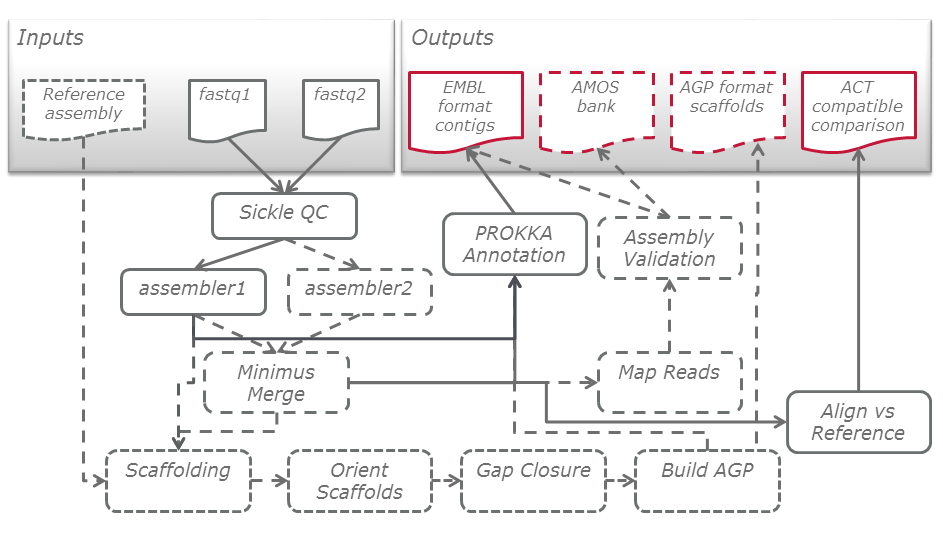
\includegraphics[width=0.9\textwidth]{workflow}}
\caption{BugBuilder Workflow}
\label{fig:BugBuilderWorkflow}
\end{figure}

The overall BugBuilder workflow is shown in Figure ~\ref{fig:BugBuilderWorkflow}. The core workflow
is indicated by solid lines, with hashed lines indicating optional or conditionally run parts of
the pipeline (i.e. depending upon availability of a reference genome sequence). 

\subsection{Sequence QC}

Sequence quality is key to obtaining good \textit{de-novo} assemblies. While early high-throughput
sequence assemblers ignored sequence quality scores, some degree of quality screening is now
incorporated into a number of assemblers. Given the variability of how assemblers cope with poor
quality sequence, BugBuilder carries out an initial screening of the submitted sequences using
the Sickle tool, trimming reads with a quality score below 20 within a sliding window. The correct
quality score encoding is first determined automatically using fastqident.

\subsection{Assembly}

The job of glueing together the huge number of sequence reads generated during a sequencing
experiment is handled by a tool known as an assembler. There are now a considerable number of
assemblers available capable of producing good assemblies from high-throughput sequencing of
microbial genomes. The assembly problem is not entirely solved, however, and new and improved
assemblers are regularly being released. Rather than base BugBuilder around a specific assembler,
it has instead been developed as a framework which various different assemblers can be plugged
into, allowing the assembly component to be readily updated as new algorithms are made available.
BugBuilder is made available with configurations for the AbySS and Spades assemblers, however
alternative assemblers may have been configured in your installation.

A list of the assemblers available within the BugBuilder installation can be obtained by running

\begin{verbatim}
[jamesa@codon ~]$ BugBuilder --help

Welcome to BugBuilder

Available assemblers: spades, abyss
Available scaffolders: SIS, sspace
\end{verbatim}

The assembler to be used can then be selected at runtime using the {\tt --assembler} command line
argument: 

\begin{verbatim}
BugBuilder --fastq1 read1.fastq --fastq2 read2.fastq  \
    --reference myreference.fasta --assembler abyss 
\end{verbatim}

If no assembler is specified on the command line, the first of those displayed on the list of
available assemblers will be used. The order of this list is controlled by the 'priority' attribute
in the 'assemblers' section of the configuration file.

\subsection{Multiple Assemblers}

Assemblers typically break contig sequences where sequences become repetitive and difficult to
extend unambiguously. Different algorithms will break contigs in different locations, hence it is
sometimes possible to get better coverage of a genome by combining multiple assemblies. BugBuilder
supports running two independent assemblers, and merging the results (using minimus from the AMOS
package). While this approach can produce better genome coverage, it does introduce an addition
means of introducing misassemblies, and can result in less contiguous assembles, albeit covering a
greater proportion of a genome. 

Running multiple assemblers simply requires the {\tt --assembler} command-line argument to be
specified twice:

\begin{verbatim}
BugBuilder --fastq1 read1.fastq --fastq2 read2.fastq  \
    --reference myreference.fasta --assembler abyss --assembler spades
\end{verbatim}

\subsection{Scaffolding}

The primary job of an assembler is to build a series of contiguous sequences from the separate
sequence reads, extending these sequences as far as possible until it becomes no longer possible to
unambiguously extend the contig sequences. Based upon the location of paired reads on different
contigs, even when it is no longer possible to extend a contig sequence any further, it can
sometimes be possible to make an association between  contigs and get an idea of the size of the
gap between them. This is a process known as scaffolding, which is undertaken by some assembly
algorithms, but which may also be carried out separately by standalone scaffolding algorithms.

If scaffolds are produced by the selected assembler, these will be available for downstream
processes, however if a standalone scaffolder is selected, the outputs of this will be used in
preference to those from the assembler. 

Scaffolding is the process through which sequence contigs can be arranged to give an impression of
the larger-scale organisation of a genome. Typically this is carried out using evidence of
association between contigs obtained from read-pairs located on different contigs (see figure
~\ref{fig:ReadPairScaffolding}). This approach tends to have limited success with bacterial genomes
sequenced with a single short-insert library since the library insert size is insufficient to span
repetitive regions within the genome. An alternative approach which has had considerable success
with microbial genomes is to align the generated contigs against the genome sequence of a closely
related organism, and use this evidence to order and orientate the contigs.

\begin{figure}[h]
\fbox{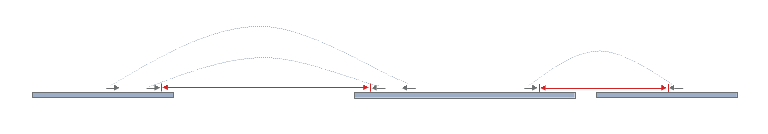
\includegraphics[width=0.9\textwidth]{paired_read_scaffolding}}
\caption{Scaffolding contigs with read-pair information}
\label{fig:ReadPairScaffolding}
\end{figure}

As with assembly algorithms, BugBuilder allows scaffolding algorithms to be preconfigured and
selected at runtime rather than tying the pipeline into one algorithm. BugBuilder is preconfigured
to work with the SSPACE and SIS scaffolders. SSPACE utilises read-pair information to generate
scaffolds, and with microbial genomes typically does not outperform the scaffolding algorithms
build into assembly tools. SIS is a tool which utilises MUMmer to align the contigs against a
reference genome, and utilises this information to determine the order and organisation of contig
sequences.  

The advantage of read-pair based scaffolding algorithms is that they are not biased by external
factors, whereas alignment against a reference genome may result in an assembly which is
artificially skewed towards the organisation of the reference organism. Reference guided
scaffolding typically produces far lower number of scaffolds, however.

\subsection{Scaffold Orientation and Origin Identification}

Some scaffolders will output scaffolds in the correct orientation, but this behaviour varies
between scaffolders, and those which just make use of read-pair information have no way of
determining the correct orientation. If a reference genome is provided, BugBuilder will then align
the scaffolds against this reference to ensure they are correctly orientated. 

Contigs produced during assembly will typically span the origin of replication. BugBuilder will
attempt to locate the origin within the assembled scaffolds based upon the reference genome
alignment, and will split the scaffolds at this point, relocating the upstream region to the other
end of the assembly.

\subsection{Gap Closure}

Once scaffolds have been ordered, it can be possible to further close some gaps between contigs
where the assembler was not able to unambiguously extend the contig. BugBuilder uses the GapFiller
tool produced by BaseClear for this stage of the workflow. GapFiller iteratively aligns reads from
the fastq files against the scaffolds, looking for read-alignments which hang off the end
of the contiguous sequences. After a number of cycles, some of these extensions may end up
spanning the gap between contigs.

\subsection{AGP Generation}

Scaffold structures for genomes submitted to public databases need to be defined in AGP ('A Golden
Path') files. This is a text file which species the order and orientation of the contigs on the
scaffolds, the sizes of the gaps between contigs and the kind of evidence used to establish the
ordering.  BugBuilder processes the scaffolds to extract fresh contig sequences by splitting the
scaffolds around 'N's. The public database require a minimum contig size of 200 bp, and do not
allow runs of more than 10 'N's in contig sequences. Contigs shorter than 200 bp are therefore
discarded, and if these are within scaffolds the scaffold gaps are extended to take account of the
removed sequence.  The type of evidence for the gaps is added according to the value of the
'linkage-evidence' attribute in the  scaffolder configuration.

\subsection{Contig Annotation}

Contigs are annotated using the Prokka package, which utilises a number of tools for
\textit{de-novo} CDS, tRNA and rRNA  identification. It uses organism specific databases to aid
the annotation and can be passed arguments to indicate the genus and species of the genome being
annotated. BugBuilder similarly allows these arguments to be specified on the command-line, using
the {\tt --genus} and {\tt --species} arguments, and passes these values to Prokka if they are provided. 

\begin{verbatim}
BugBuilder --fastq1 read1.fastq --fastq2 read2.fastq  \
    --reference myreference.fasta --genus Streptococcus --species pyogenes
\end{verbatim}

Prokka post-processes the annotations to identify terms which do not conform to the NCBI
recommendations, and corrects these. 

\subsection{Reference alignment}

BugBuilder also carries out alignments of the scaffolds against the reference genome (if provided)
using BLAST, and output in a format appropriate for viewing with the Artemis Comparison Tool (ACT).
A second alignment is carried out using MUMmerplot to provide an overview of how the assembly
compares with the reference.  

\subsection{Outputs}

The resulting output files are copied into a directory within the directory from which BugBuilder
was launched. If genus/species/strain names have been provided, the directory will be named {\tt
BugBuilder\_genus\_species\_strain}. If the full contents of the working directory are required, for
example for debugging purposes, specifiying the {\tt --keepall} command-line argument will copy the
full contents of the directory rather than just the final output files.

\section{Submission vs Finishing Modes}

BugBuilder can be run in modes targeted at producing output suitable for submission to public
databases, or for carrying out further finishing work. The mode to run in is defined using the {\tt
--mode} command line argument, which accepts values of either 'submission' or 'finishing'. The
default mode is 'submission'.

\subsection{Submission Mode}

Submission mode creates output suitable for submission to the ENA, with contigs \textless200 bp removed,
and no consecutive runs of more than 10 'N's in contig sequences. This is the default mode. 

\subsection{Finishing Mode}

Finishing mode does not remove short contig sequences from the assembly, retaining the full output
of the assembler. In order to highlight potential areas of misassembly, the amosvalidate tool from
the AMOS package is run against the assembly. This first requires the sequence reads to be mapped
against the assembly, since the majority of assemblers do not track the placement of reads in an
assembly. Amosvalidate analyses the read-placements and identifies features such as read-pairs
which are separated by a distance outlying the normal distribution of the library or regions of
unusually high read coverage (potentially indicative of a collapsed repeat region). These results
are stored in Amos's bank format, which can be viewed using the Hawkeye viewer. The AMOS bank is
not returned in the default set of results, so if this is required, the {\tt --keepall}
command-line argument also needs to be specified. The results are also parsed and included in the
EMBL format report, allowing them to be viewed in the context of the annotations e.g. using
Artemis.

Please note that there are always likely to be false-positives in the issues reported, for example
by definition, a small proportion of mate-pairs are always going to be outside the
standard-deviation of the insert-size for the library. The requirement to map the reads against the
assembly is itself potentially a source of error. The mapped location of a read is not necessarily
that which was used in the assembly process. The most frequent regions containing misassemblies are
those around repeats, where the read-mapping process is likely to be least accurate. 

\section{The Working Directory}

A separate working directory is created for each job within the 'tmp\_dir' defined within the
BugBuilder configuration. Once the job starts, the fastq files and reference genome are copied to
the this directory, and all subsequent operations carried out within it.  This is intended to make
the system readily amenable to running on a cluster.  Each separate component of the pipeline
creates it's own subdirectory within the working directory to keep it's files in. 
A series of symbolic links are created and updated within this directory as the pipeline
progresses, pointing toward the latest verisons of each of these files within the subdirectories.
This directory is automatically deleted once the job has completed, however a failed job will
typically result in the directory being left with the temporary directory.


\section{Command Reference}

The following command reference is generated from the embedded documentation in BugBuilder. 

\include{command_reference}
\end{document}
